% !TEX program = pdflatex
% Quantum Mechanics Homework_4
\documentclass[12pt,a4paper]{article}
\usepackage[top=1in,bottom=1in,left=.5in,right=.5in]{geometry} 
\usepackage{amsmath,amsthm,amssymb,amsfonts,enumitem,fancyhdr,color,comment,graphicx,environ}
\pagestyle{fancy}
\setlength{\headheight}{65pt}
\newenvironment{problem}[2][Problem]{\begin{trivlist}
\item[\hskip \labelsep {\bfseries #1}\hskip \labelsep {\bfseries #2.}]}{\end{trivlist}}
\newenvironment{sol}
    {\emph{Solution:}
    }
    {
    \qed
    }
\specialcomment{com}{ \color{blue} \textbf{Comment:} }{\color{black}} %for instructor comments while grading
\NewEnviron{probscore}{\marginpar{ \color{blue} \tiny Problem Score: \BODY \color{black} }}
\usepackage[UTF8]{ctex}
\lhead{Name: 陈稼霖\\ StudentID: 45875852}
\rhead{PHYS1501 \\ Quantum Mechanics \\ Semester Fall 2019 \\ Assignment 4}
\begin{document}
\begin{problem}{1}
[C-T Exercise 1-7] Consider a particle of mass $m$ placed in the one-dimensional potential
\begin{equation}
V(x)=
\left\{\begin{array}{ll}
\infty,&x<0,\\
-V_0,&0\leq x\leq a,\\
0,&x\geq a.
\end{array}\right.
\end{equation}
Let $\varphi(x)$ be a wave function associated with a stationary state of the particle.
\begin{itemize}
\item[(a)] Show that $\varphi(x)$  can be extended to give an odd wave function which corresponds to a stationary state for a square well of width $2a$ and depth $V_0$.
\item[(b)]  Discuss, with respect to $a$ and $V_0$, the number of bound states of the particle. Is there always at least one such state as for the symmetric square well?
\end{itemize}
\end{problem}
\begin{sol}
\begin{itemize}
\item[(a)] For the particle placed in the one-dimensional potential described in the problem, at $x<0$, since $V(x)=\infty$, the wavefunction
\begin{equation}
\varphi(x)=0,\quad x<0
\end{equation}
For a particle of mass $m$ placed in the one-dimensional potential as mentioned in the problem, at $0\leq x\leq a$, let $k=\sqrt{\frac{2m(E+V_0)}{\hbar^2}}$, the general solution of wavefunction
\begin{equation}
\varphi(x)=A\sin kx,\quad 0\leq x\leq a
\end{equation}
At $x>a$, let $\kappa=\sqrt{\frac{2mE}{\hbar^2}}$, the general solution of wavefunction
\begin{equation}
\varphi(x)=Be^{-\kappa x},\quad x>a
\end{equation}
The matching condition
\begin{gather}
\varphi(a^-)=A\sin ka=\varphi(a^+)=Be^{-\kappa a}\\
\varphi'(a^-)=Ak\cos ka=\varphi'(a^+)=-B\kappa e^{-\kappa a}
\end{gather}
give
\begin{gather}
B=Ae^{\kappa a}\sin ka\\
\label{energies}-\frac{k}{\kappa}=\tan ka
\end{gather}
Therefore, the wavefunction (without normalization) is
\begin{equation}
\varphi(x)=
\left\{\begin{array}{ll}
0,&x<0\\
A\sin ka,&0\leq x\leq a\\
Ae^{\kappa(a-x)}\sin ka,&x>a
\end{array}\right.
\end{equation}
Extend the wavefunction to give an odd function
\begin{equation}
\varphi(x)=
\left\{\begin{array}{ll}
A\sin kx,&|x|\leq a\\
Ae^{-\kappa|x-a|}\sin ka,&x>a
\end{array}\right.
\end{equation}
which corresponds to a stationary state for a square well of width $2a$ and depth $V_0$.
\item[(b)] The energies of bound states satisfy equation (\ref{energies}). Let $k_0=\sqrt{\frac{2mV_0}{\hbar^2}}$, rewrite equation (\ref{energies}) (note that $k>0$, $k_0>0$)
\begin{equation}
\sin ka=\pm\frac{ka}{k_0a},\quad(ka\text{ is at the second or forth quadrant})
\end{equation}
Therefore, the number of bound states of the particle equals the number of intersections of $ka/k_0a$ and $|\sin ka|$ at the second or forth quadrant
\begin{equation}
\text{the number of bound states}=\left[\frac{k_0a}{\pi}+\frac{1}{2}\right]=\left[\frac{a\sqrt{2mV_0}}{\pi\hbar}+\frac{1}{2}\right]
\end{equation}
where $[n]$ is the maximum integer less than $n$, as shown in fig \ref{problem_1}.
\begin{figure}[h]
\centering
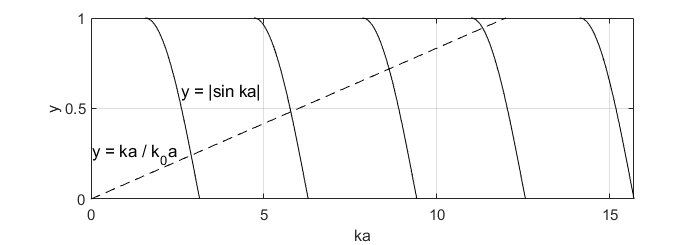
\includegraphics[scale=.8]{problem_1.png}
\caption{The number of bound state equals the number of intersections of $ka/k_0a$ and $|\sin ka|$ at the second or forth quadrant}\label{problem_1}
\end{figure}
\\The condition for existence of (at least one) bound states is
\begin{equation}
k_0a>\frac{\pi}{2}\Longrightarrow V_0a^2\geq\frac{\pi^2\hbar^2}{8m}
\end{equation}
The condition for existence and the number of odd bound states for the symmetric square well is the same as calculated above. However, there is always at least one even bound state for the symmetric square well.
\end{itemize}
\end{sol}

\begin{problem}{2}
Consider a particle of mass $m$ placed in the one-dimensional potential
\[
V(x)=
\left\{\begin{array}{ll}
\lambda\delta(x),&|x|<a,\\
\infty,&|x|\geq a.
\end{array}\right.
\]
Here $\lambda>0$. Find the energies and wave functions of the stationary states for the particle. The wave functions are not required to be normalized.
\end{problem}
\begin{sol}
At $|x|>a$, since $V(x)=\infty$, the wavefunction
\begin{equation}
\varphi(x)=0,\quad|x|>0
\end{equation}
Let $k=\sqrt{\frac{2mE}{\hbar^2}}$. At $-a<x<0$, since $\varphi(-a^+)=\varphi(-a^-)=0$, the general solution of wavefunction
\begin{equation}
\varphi(x)=A\sin k(a+x),\quad-a<x<0
\end{equation}
At $0<x<a$, since $\varphi(a^-)=\varphi(a^+)=0$, the general solution of wavefunction
\begin{equation}
\varphi(x)=B\sin k(a-x),\quad0<x<a
\end{equation}
The matching condition
\small\begin{gather}
\varphi(0^-)=A\sin ka=\varphi(0^+)=B\sin ka\\
\varphi'(0^+)-\varphi'(0^-)=-kA\cos ka+kB\cos ka=\lim_{\epsilon\rightarrow0}\int_{-\epsilon}^{+\epsilon}-\frac{2m}{\hbar^2}(E-V)\varphi(x)dx=\frac{2m\lambda}{\hbar^2}\varphi(0)
\end{gather}\normalsize
gives
\begin{gather}
\left\{\begin{array}{l}
B=A\\
-\frac{\hbar^2k}{m\lambda}=\tan ka
\end{array}\right.(\text{even parity states})\\
\left\{\begin{array}{l}
B=-A\\
k=\frac{n\pi}{a},\quad n=1,2,\cdots
\end{array}\right.(\text{odd parity states})
\end{gather}
Therefore, the wavefunction of even parity stationary states is
\begin{equation}
\varphi(x)=\left\{\begin{array}{ll}
A\sin k(x+a),&-a<x<0\\
A\sin k(x-a),&0<x<a\\
0,&|x|\geq a
\end{array}\right.
\end{equation}
where $A$ is the normalization constant and its energies is determined by
\begin{equation}
-\frac{\hbar^2k}{m\lambda}=\tan ka\Longrightarrow-\frac{\hbar^2\sqrt{2mE}}{m\lambda}=\tan\frac{a\sqrt{2mE}}{\hbar}
\end{equation}
the wavefunction of odd parity stationary states is
\begin{equation}
\varphi(x)=\left\{\begin{array}{ll}
A\sin\frac{n\pi x}{a},&|x|<a\\
0,&|x|\geq a
\end{array}\right.
\end{equation}
where $A$ is the normalization and its energies are
\begin{equation}
E_n=\frac{n^2\pi^2\hbar^2}{2ma^2},\quad n=1,2,\cdots
\end{equation}
\end{sol}

\begin{problem}{3}
Consider a particle of mass $m$ placed in the one-dimensional potential
\[
V(x)=
\left\{\begin{array}{ll}
V_1,&x\leq0,\\
0,&0<x<a,\\
V_2,&x\geq a.
\end{array}\right.
\]
Here $V_1>V_2$. Find the equation that determines the energies of the bound states of the particle.
\end{problem}
\begin{sol}
At $x\leq0$, let $k_1=\sqrt{\frac{2m(V_1-E)}{\hbar^2}}$, the general solution of bound state wavefunction
\begin{equation}
\varphi(x)=Ae^{k_1x},\quad x\leq0
\end{equation}
At $0<x<a$, let $k=\sqrt{\frac{2mE}{\hbar^2}}$, the general solution of bound state wavefunction
\begin{equation}
\varphi(x)=B\cos kx+C\sin kx,\quad0<x<a
\end{equation}
At $x\geq a$, let $k_2=\sqrt{\frac{2m(V_2-E)}{\hbar^2}}$, the general solution of bound state wavefunction
\begin{equation}
\varphi(x)=De^{-k_2(x-a)},\quad x\geq a
\end{equation}
The matching conditions
\begin{gather}
\varphi(0^-)=A=\varphi(0^+)=B\\
\varphi(a^-)=B\cos ka+C\sin ka=\varphi(a^+)=D\\
\varphi'(0^-)=Ak_1=\varphi(0^+)=Ck\\
\varphi'(a^-)=-Bk\sin ka+Ck\cos ka=\varphi(a^+)=-Dk_2
\end{gather}
give
\begin{gather}
B=A\\
C=\frac{k_1A}{k}\\
D=(\cos ka+\frac{k_1}{k}\sin ka)A\\
\frac{(k_1+k_2)k}{k^2-k_1k_2}=\tan ka
\end{gather}
The equation that determines the energy of the bound states of the particle is
\begin{equation}
\frac{(k_1+k_2)k}{k^2-k_1k_2}=\tan ka,\quad\quad(E<E_2)
\end{equation}
where $k=\sqrt{\frac{2mE}{\hbar^2}}$, $k_1=\sqrt{\frac{2m(V_1-E)}{\hbar^2}}$, $k_2=\sqrt{\frac{2m(V_2-E)}{\hbar^2}}$.
\end{sol}

\begin{problem}{4}
Consider a particle of mass $m$ placed in a one-dimensional infinite-depth potential well with the potential energy given by
\[
V(x)=
\left\{\begin{array}{ll}
0,&0<x<a,\\
\infty,&x\leq0,x\geq a.
\end{array}\right.
\]
The particle is in a state described by the wave function $\psi(x)=Ax(x-a)\theta(x)\theta(a-x)$ with $A=\sqrt{30}a^{-5/2}$.
\begin{itemize}
\item[(a)] If the energy of the particle is measured, what are the possible results? What are the probabilities of obtaining these results?
\item[(b)] What is the mean of all possible experimental results when the energy of the particle is measured? What is the standard deviation?
\end{itemize}
\end{problem}
\begin{sol}
\begin{itemize}
\item[(a)] The eigenfunctions of the particle in the one-dimensional infinite-depth potential well is
\begin{equation}
\varphi_n(x)=\sqrt{\frac{2}{a}}\sin\left(\frac{n\pi x}{a}\right)\theta(x)\theta(a-x),\quad n=1,2,\cdots
\end{equation}
whose corresponding energies are
\begin{equation}
E_n=\frac{n^2\pi^2\hbar^2}{2ma^2},\quad n=1,2,\cdots
\end{equation}
Expansion of the wavefunction
\begin{equation}
\psi(x)=\sum_{i=1}^{\infty}c_n\varphi_n(x)
\end{equation}
Expansion coefficients
\begin{align}
\nonumber c_n(x)=&\int_{-\infty}^{+\infty}\varphi_n^*(x)\psi(x)dx\\
=&\int_{-\infty}^{+\infty}-\sqrt{\frac{2}{a}}\sin\left(\frac{n\pi x}{a}\right)\cdot Ax(x-a)\theta(x)\theta(a-x)dx\\
\nonumber=&-\sqrt{\frac{2}{a}}A\int_0^a(x^2-ax)\sin\left(\frac{n\pi x}{a}\right)dx\\
\nonumber=&\sqrt{\frac{2}{a}}A\frac{a}{n\pi}\int_0^a(x^2-ax)d\cos\left(\frac{n\pi x}{a}\right)\\
\nonumber=&\sqrt{\frac{2}{a}}A\frac{a}{n\pi}\left[\left.(x^2-ax)\cos\left(\frac{n\pi x}{a}\right)\right|_0^a-\int_0^a\cos\left(\frac{n\pi x}{a}\right)dx(x-a)\right]\\
\nonumber=&-\sqrt{\frac{2}{a}}A\frac{a}{n\pi}\int_0^a(2x-a)\cos\left(\frac{n\pi x}{a}\right)dx\\
\nonumber=&-\sqrt{\frac{2}{a}}A\left(\frac{a}{n\pi}\right)^2\int_0^a(2x-a)d\sin\left(\frac{n\pi x}{a}\right)\\
\nonumber=&-\sqrt{\frac{2}{a}}A\left(\frac{a}{n\pi}\right)^2\left[\left.(2x-a)\sin\left(\frac{n\pi x}{a}\right)\right|_0^a-\int_0^a\sin\left(\frac{n\pi x}{a}\right)d(2x-a)\right]\\
\nonumber=&\sqrt{\frac{2}{a}}A\left(\frac{a}{n\pi}\right)^22\int_0^a\sin\left(\frac{n\pi x}{a}\right)dx\\
\nonumber=&\sqrt{\frac{2}{a}}A\left(\frac{a}{n\pi}\right)^32[1-(-1)^n]\\
=&\frac{4\sqrt{15}}{(n\pi)^3}[1-(-1)^n]=\left\{\begin{array}{ll}\frac{8\sqrt{15}}{(n\pi)^3},&n\text{ is odd}\\0,&n\text{ is even}\end{array}\right.
\end{align}
The probability of obtaining the result $E_n$ is
\begin{equation}
P_n=c_n^2=\frac{240}{(n\pi)^6}[1-(-1)^n]^2=\left\{\begin{array}{ll}\frac{960}{(n\pi)^6},&n\text{ is odd}\\0,&n\text{ is even}\end{array}\right.
\end{equation}
Therefore, the possible results are
\begin{equation}
E_n=\frac{n^2\pi^2\hbar^2}{2ma^2},\quad n=1,3,5,\cdots
\end{equation}
with probability
\begin{equation}
P_n=\frac{960}{(n\pi)^6},\quad n=1,3,5,\cdots
\end{equation}
to be obtained.
\item[(b)] The mean of all possible experiment results
\begin{equation}
\langle E\rangle=\sum_{n=1,3,5,\cdots}E_nP_n=\sum_{n=1,3,5,\cdots}\frac{n^2\pi^2\hbar^2}{2ma^2}\cdot\frac{960}{(n\pi)^6}=\frac{480\hbar^2}{\pi^4ma^2}\sum_{n=1,3,5,\cdots}\frac{1}{n^4}
\end{equation}
To calculate $\sum_{n=1,3,5,\cdots}\frac{1}{n^4}$, first calculate $\sum_{i=1}^{\infty}\frac{1}{n^4}$ with Fourier series
\begin{align}
\nonumber x^4-2\pi^2x^2=&\frac{1}{2\pi}\int_{-\pi}^{\pi}(x^4-2\pi^2x^2)dx+\sum_{n=1}^{\infty}\left[\frac{2}{\pi}\int_0^{\pi}(x^4-2\pi^2x^2)\cos nxdx\right]\cos nx\\
\nonumber=&-\frac{7\pi^4}{15}+\sum_{n=1}^{\infty}\frac{2}{n\pi}\left[\int_0^{\pi}(x^4-2\pi^2x^2)d\sin nx\right]\cos nx\\
\nonumber=&-\frac{7\pi^4}{15}+\sum_{n=1}^{\infty}\frac{2}{n\pi}\left[\left.(x^4-2\pi^2x^2)\sin nx\right|_0^{\pi}-\int_0^{\pi}\sin nxd(x^4-2\pi^2x^2)\right]\cos nx\\
\nonumber=&-\frac{7\pi^4}{15}-\sum_{n=1}^{\infty}\frac{2}{n\pi}\left[\int_0^{\pi}(4x^3-4\pi^2x)\sin nxdx\right]\cos nx\\
\nonumber=&-\frac{7\pi^4}{15}+\sum_{n=1}^{\infty}\frac{2}{n^2\pi}\left[\int_0^{\pi}(4x^3-4\pi^2x)d\cos nx\right]\cos nx\\
\nonumber=&-\frac{7\pi^4}{15}+\sum_{n=1}^{\infty}\frac{2}{n^2\pi}\left[\left.(4x^3-4\pi^2x)\cos nx\right|_0^{\pi}-\int_0^{\pi}\cos nxd(4x^3-4\pi^2x)\right]\cos nx\\
\nonumber=&-\frac{7\pi^4}{15}-\sum_{n=1}^{\infty}\frac{2}{n^2\pi}\left[\int_0^{\pi}(12x^2-4\pi^2)\cos nxdx\right]\cos nx\\
\nonumber=&-\frac{7\pi^4}{15}-\sum_{n=1}^{\infty}\frac{2}{n^3\pi}\left[\int_0^{\pi}(12x^2-4\pi^2)d\sin nx\right]\cos nx\\
\nonumber=&-\frac{7\pi^4}{15}-\sum_{n=1}^{\infty}\frac{2}{n^3\pi}\left[\left.(12x^2-4\pi^2)\sin nx\right|_0^{\pi}-\int_0^{\pi}\sin nxd(12x^2-4\pi^2)\right]\cos nx\\
\nonumber=&-\frac{7\pi^4}{15}+\sum_{n=1}^{\infty}\frac{2}{n^3\pi}\left[\int_0^{\pi}24x\sin nxdx\right]\cos nx\\
\nonumber=&-\frac{7\pi^4}{15}+\sum_{n=1}^{\infty}\frac{2}{n^4\pi}\left[\int_0^{\pi}24xd\cos nx\right]\cos nx\\
\nonumber=&-\frac{7\pi^4}{15}-\sum_{n=1}^{\infty}\frac{2}{n^4\pi}\left[\left.24x\cos nx\right|_0^{\pi}-\int_0^{\pi}\cos nxd(24x)\right]\cos nx\\
=&-\frac{7\pi^4}{15}-\sum_{n=1}^{\infty}\frac{48(-1)^n}{n^4}\cos nx
\end{align}
Let $x=\pi$, then
\begin{gather}
\Longrightarrow\sum_{n=1}^{\infty}\frac{1}{n^4}=\frac{\pi^4}{90}\\
\Longrightarrow\sum_{n=2,4,6,\cdots}\frac{1}{n^4}=\frac{1}{2^4}\sum_{n=1}^{\infty}\frac{1}{n^4}=\frac{\pi^4}{1440}\\
\Longrightarrow\sum_{n=1,3,5,\cdots}\frac{1}{n^4}=\sum_{n=1}^{\infty}\frac{1}{n^4}-\sum_{n=2,4,6,\cdots}\frac{1}{n^4}=\frac{\pi^4}{960}
\end{gather}
Therefore, the mean of all possible experiment results
\begin{equation}
\langle E\rangle=\frac{480\hbar^2}{\pi^4ma^2}\sum_{n=1,3,5,\cdots}\frac{1}{n^4}=\frac{\hbar^2}{2ma^2}
\end{equation}
The square mean
\begin{equation}
\langle E^2\rangle=\sum_{n=1,3,5,\cdots}E_n^2P_n=\sum_{n=1,3,5,\cdots}\left(\frac{n^2\pi^2\hbar^2}{2ma^2}\right)^2\cdot\frac{960}{(n\pi)^6}=\frac{240\hbar^4}{\pi^2ma^2}\sum_{n=1,3,5,\cdots}\frac{1}{n^2}
\end{equation}
To calculate $\sum_{n=1,3,5}$, first calculate $\sum_{n=1}^{\infty}\frac{1}{n^2}$ with Fourier series
\begin{align}
\nonumber x^2=&\frac{1}{2\pi}\int_{-\pi}^{\pi}x^2dx+\sum_{n=1}^{\infty}\left[\frac{2}{\pi}\int_0^{\pi}x\cos nxdx\right]\cos nx\\
\nonumber=&\frac{\pi^2}{3}+\sum_{n=1}^{\infty}\frac{2}{n\pi}\left[\int_0^{\pi}x^2d\sin nx\right]\cos nx\\
\nonumber=&\frac{\pi^2}{3}+\sum_{n=1}^{\infty}\frac{2}{n\pi}\left[\left.x^2\sin nx\right|_0^{\pi}-\int_0^{\pi}\sin nxdx^2\right]\cos nx\\
\nonumber=&\frac{\pi^2}{3}-\sum_{n=1}^{\infty}\frac{4}{n\pi}\left[\int_0^{\pi}x\sin nxdx\right]\cos nx\\
\nonumber=&\frac{\pi^2}{3}+\sum_{n=1}^{\infty}\frac{4}{n^2\pi}\left[\int_0^{\pi}xd\cos nx\right]\cos nx\\
\nonumber=&\frac{\pi^2}{3}+\sum_{n=1}^{\infty}\frac{4}{n^2\pi}\left[\left.x\cos nx\right|_0^{\pi}-\int_0^{\pi}\cos nxdx\right]\cos nx\\
=&\frac{\pi^2}{3}+\sum_{n=1}^{\infty}\frac{4(-1)^n}{n^2}\cos nx
\end{align}
Let $x=\pi$, then
\begin{gather}
\Longrightarrow\sum_{n=1}^{\infty}\frac{1}{n^2}=\frac{\pi^2}{6}\\
\Longrightarrow\sum_{n=2,4,6,\cdots}\frac{1}{n^2}=\frac{1}{4}\sum_{n=1}^{\infty}\frac{1}{n^2}=\frac{\pi^2}{24}\\
\Longrightarrow\sum_{n=1,3,5,\cdots}\frac{1}{n^2}=\sum_{n=1}^{\infty}\frac{1}{n^2}-\sum_{n=2,4,6,\cdots}\frac{1}{n^2}=\frac{\pi^2}{8}\\
\Longrightarrow\langle E^2\rangle=\frac{240\hbar^4}{\pi^2ma^2}\sum_{n=1,3,5,\cdots}\frac{1}{n^2}=\frac{30\hbar^4}{ma^2}
\end{gather}
Therefore, the standard deviation of the experimental results is
\begin{equation}
\sigma(E)=\sqrt{\langle E^2\rangle-\langle E\rangle^2}=\frac{\sqrt{119}\hbar^2}{2\sqrt{m}a}
\end{equation}
\end{itemize}
\end{sol}

\begin{problem}{5}
[C-T Exercise 1-5] Consider a particle of mass $m$ whose potential energy is $V(x)=-\alpha\delta(x)-\alpha\delta(x-l)$, where $\alpha$ is greater than zero and $l$ is a constant length.
\begin{itemize}
\item[(a)] Calculate the bound states of the particle, setting $E=-\frac{\hbar^2\rho^2}{2m}$. Show that the possible energies are given by the relation $e^{-\rho l}=\pm\left(1-\frac{2\rho}{\mu}\right)$ with $\mu=\frac{2m\alpha}{\hbar^2}$. Give a graphic solution of this equation.
\begin{itemize}
\item[i.] \textit{Ground state.} Show that this state is even (invariant with respect to reflection about the point $x=l/2$), and that its energy $E_S$ is less than the energy $-E_L=-\frac{m\alpha^2}{2\hbar^2}$. Interpret this result physically. Represent graphically the corresponding wave function.
\item[ii.] \textit{Excited state.} Show that, when $l$ is greater than a value which you are to specify, there exists an odd excited state of energy $E_A$ greater than $-E_L$. Find the corresponding wave function.
\item[iii.] Explain how the preceding calculations enable us to construct a model which represents an ionized diatomic molecule (H$_2^+$, for example) whose nuclei are separated by a distance $l$.  How do the energies of the two levels vary with respect to $l$? What happens at the limit where $l\rightarrow0$ and at the limit where $l\rightarrow\infty$? If the repulsion of the two nuclei is taken into account, what is the total energy of the system? Show that the curve which gives the variation with respect to $l$  of the energies thus obtained enables us to predict in certain cases the existence of bound states of H$_2^+$, and to determine the value
of $l$ at equilibrium. In this way we obtain a very elementary model of the chemical bond.
\end{itemize}
\item[(b)] Calculate the reflection and transmission coefficients of the system of two delta function barriers. Study their variations with respect to $l$. Do the resonances thus obtained occur when $l$ is an integral multiple of the de Broglie wavelength of the particle? Why?
\end{itemize}
\end{problem}
\begin{sol}
\begin{itemize}
\item[(a)] At $x<0$, the general solution of the wavefunction
\begin{equation}
\varphi(x)=Ae^{\rho x}
\end{equation}
At $0\leq x\leq l$, the general solution of the wavefunction
\begin{equation}
\varphi(x)=Be^{\rho x}+Ce^{-\rho x}
\end{equation}
At $x>l$, the general solution of the wavefunction
\begin{equation}
\varphi(x)=De^{-\rho x}
\end{equation}
The matching conditions
\begin{gather}
\varphi(0^-)=A=\varphi(0^+)=B+C\\
\varphi(l^-)=Be^{\rho l}+Ce^{-\rho l}=\varphi(l^+)=De^{-\rho l}\\
\varphi'(0^+)-\varphi'(0^-)=B\rho-C\rho-A\rho=-\frac{2m\alpha}{\hbar^2}\varphi(0)=-\mu A\\
\varphi'(l^+)-\varphi'(l^-)=-D\rho e^{-\rho l}-(B\rho e^{\rho l}-C\rho e^{-\rho l})=-\frac{2m\alpha}{\hbar^2}\varphi(l)=-\mu De^{-\rho l}
\end{gather}
give
\begin{gather}
B=\left(1-\frac{\mu}{2\rho}\right)A\\
C=\frac{\mu}{2\rho}A\\
D=\left[\left(1-\frac{\mu}{2\rho}\right)e^{2\rho l}+\frac{\mu}{2\rho}\right]A\\
e^{-\rho l}=\left(1-\frac{2\rho}{\mu}\right)^2
\end{gather}
Therefore, the possible energies are given by the relation
\begin{equation}
e^{-\rho l}=\pm\left(1-\frac{2\rho}{\mu}\right)
\end{equation}
Graphic solution
\begin{figure}[h]
\centering
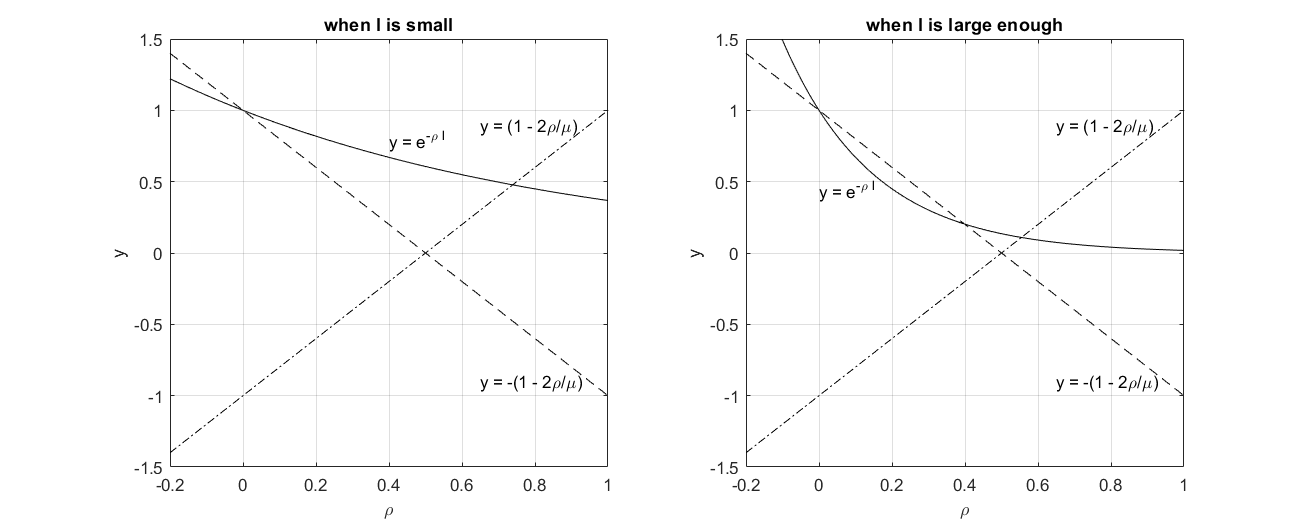
\includegraphics[scale=0.5]{problem_5.png}
\caption{Possible energies of the bound states are given by the relation $e^{-\rho l}=\pm\left(1-\frac{2\rho}{\mu}\right)$}\label{problem_5}
\end{figure}
\\The possible energies is corresponding to $y=e^{-\rho l}$'s intersection point with $y=-(1-\frac{2\rho}{\mu})$ and $y=(1-\frac{2\rho}{\mu})$ (the intersection point $\rho=0$ means $E=0$ which is not the energy of bound state and should be discarded).
\begin{itemize}
\item[i.] According to figure \ref{problem_5}, the energy of ground state is $E_S=-\frac{\hbar^2\rho^2}{2m}$, whose $\rho$ is given by the relation $e^{-\rho l}=-(1-\frac{2\rho}{\mu})$ so the wavefunction
\begin{equation}
\varphi(x)=
\left\{\begin{array}{ll}
Ae^{\rho x},&x<0\\
A\frac{e^{\rho(x-l)+e^{-\rho x}}}{e^{-\rho l}+1},&0\leq x\leq l\\
Ae^{\rho(l-x)},&x>l
\end{array}\right.
\end{equation}
Since
\begin{equation}
\varphi(l-x)=
\left\{\begin{array}{ll}
Ae^{\rho x},&x<0\\
A\frac{e^{-\rho x}+e^{-\rho(l-x)}}{e^{-\rho l}+1},&0\leq x\leq l\\
Ae^{\rho(l-x)},&x>l
\end{array}\right.
=\varphi(x)
\end{equation}
the ground state is even.\\
Since
\begin{gather}
-1+\frac{2\rho}{\mu}=e^{-\rho l}>0\\
\Longrightarrow\rho>\frac{\mu}{2}=\frac{m\alpha}{\hbar^2}\\
\Longrightarrow E_S-(-E_L)=-\frac{\hbar^2\rho^2}{2m}+\frac{m\alpha^2}{2\hbar^2}<-\frac{m\alpha^2}{2\hbar^2}+\frac{m\alpha^2}{2\hbar^2}=0
\end{gather}
the energy of the ground state $E_S=-\frac{\hbar^2\rho^2}{2m}$ is less than the energy $-E_L=-\frac{m\alpha^2}{2\hbar^2}$.

Physically speaking, $E_S=-\frac{\hbar^2\rho^2}{2m}$ is the energy of ground state of the particle in double $\delta$-function potential well and $-E_L=-\frac{\hbar^2\rho^2}{2m}$ is the energy of ground state of the particle in single $\delta$-function potential well. Since the spatial unceritainty of the particle in double $\delta$-function potential well is greater than that in single $\delta$-function potential well, according to the uncertainty principle, the momentum uncertainty of the particle in double $\delta$-function potential well should be less than that in single $\delta$-function potential well, so be their ground state energies.

The corresponding wavefunction
\begin{figure}[h]
\centering
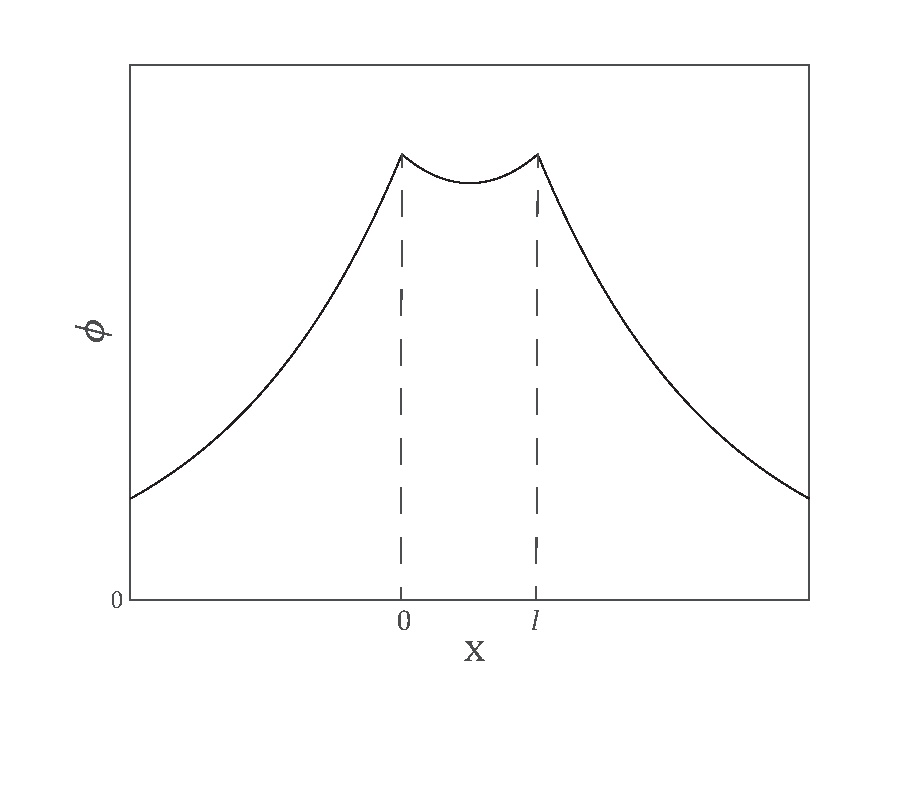
\includegraphics[scale=.5]{problem_51.eps}
\caption{The corresponding wavefunction of the particle in double $\delta$-function potential well}\label{problem_51}
\end{figure}
\newpage
\item[ii.] When the derivative of $y=e^{-\rho l}$ is less than $y=(1-\frac{2\rho}{\mu})$ at $\rho=0$, which gives
\begin{equation}
(e^{-\rho l})'|_{\rho=0}=-l<(1-\frac{2\rho}{\mu})'=-\frac{2}{\mu}\Longrightarrow l>\frac{2}{\mu},
\end{equation}
there will be another intersection point of $y=e^{-\rho l}$ and $y=(1-\frac{2\rho}{\mu})$. This intersection point is corresponding to the excited state, whose energy $E_A=-\frac{\hbar^2\rho^2}{2m}$ is given by the relation $e^{-\rho l}=(1-\frac{2\rho}{\mu})$. Since
\begin{gather}
1-\frac{2\rho}{\mu}=e^{-\rho l}>0\\
\Longrightarrow\rho<\frac{m\alpha}{\hbar^2}\\
\Longrightarrow E_A-(-E_L)=-\frac{\hbar^2\rho^2}{2m}+\frac{m\alpha^2}{2\hbar^2}>-\frac{m\alpha^2}{2\hbar^2}+\frac{m\alpha^2}{2\hbar^2}=0
\end{gather}
The energy of the state $E_A=-\frac{\hbar^2\rho^2}{2m}$ is greater than the $-E_L$.\\
The corresponding wavefunction is
\begin{equation}
\varphi(x)=
\left\{\begin{array}{ll}
Ae^{\rho x},&x<0\\
A\frac{-e^{\rho(x-l)}+e^{-\rho x}}{1-e^{-\rho l}},&0\leq x\leq l\\
-Ae^{\rho(l-x)},&x>l
\end{array}\right.
\end{equation}
Since
\begin{equation}
\varphi(l-x)=
\left\{\begin{array}{ll}
-Ae^{\rho x},&x<0\\
A\frac{-e^{-\rho x}+e^{\rho(x-l)}}{1-e^{-\rho l}},&0\leq x\leq l\\
Ae^{\rho(l-x)},&x>l
\end{array}\right.
=-\varphi(x)
\end{equation}
the excited state is odd.
\item[iii.] For an ionized diatomic molecule, H$_2^+$, for example, whose nuclei are seperated by a distance $l$, on the axis through the two nuclei, the potential energy is
\begin{equation}
V(x)=\frac{2e^2}{4\pi\epsilon_0}\left(\frac{1}{x}+\frac{1}{x-l}\right)
\end{equation}
which, for simplicity, can be treated as a double $\delta$-function potential well
as the preceding calculation dealt with.\\
When $l<\frac{2}{\mu}$, there is only a ground state. When $l>\frac{2}{\mu}$, another excited state will emerge. As $l$ becomes larger, the energy of the ground state decreases and the energy of the excited state increase.\\
At the limit where $l\rightarrow0$, the potential energy will become a single $\delta$-function and there will only be a ground state, whose energy is
\begin{equation}
e^{0}=1=-(1-\frac{2\rho}{\mu})\Longrightarrow\rho=\mu\Longrightarrow E=-\frac{2m\alpha^2}{\hbar^2}
\end{equation}
At the limit where $l\rightarrow\infty$, the ground state and the excited state will mix with each other, whose energies are both
\begin{equation}
e^{\infty}=0=(1-\frac{2\rho}{\mu})\Longrightarrow\rho=\frac{\mu}{2}\Longrightarrow E=-\frac{m\alpha^2}{2\hbar^2}
\end{equation}
Taking the repulsion of the two nuclei into account, the total energy of the system is
\begin{equation}
E_{\text{tot}}=-\frac{\hbar^2\rho^2}{2m}+\frac{e^2}{4\pi\epsilon_0l^2}
\end{equation}
where $\rho$ is given by the relation $e^{-\rho l}=\pm(1-\frac{2\rho}{\mu})$.\\
At the limit where $l\rightarrow0$, $E_{\text{tot}}\rightarrow+\infty$. At the limit where $l\rightarrow\infty$, $E_{\text{tot}}\rightarrow-\frac{2m\alpha^2}{\hbar^2}$. The energies of the system is continuous as $l$ varies, so there must be a minimum point of energies. Therefore, from curve which give the variation with respect to $l$ of the energies, the $l$ corresponding to the minimun energy is the $l$ at equilibrium.
\end{itemize}
\item[(b)] Let the incident wave come from the left side. At $x<0$, the general solution of the wavefunction
\begin{equation}
\varphi(x)=Fe^{i\rho x}+Ge^{-i\rho x}
\end{equation}
At $0\leq x\leq l$, the general solution of the wavefunction
\begin{equation}
\varphi(x)=He^{i\rho x}+Ie^{-i\rho x}
\end{equation}
At $x>l$, the general solution of the wavefunction
\begin{equation}
\varphi(x)=Je^{i\rho(x-l)}
\end{equation}
The matching conditions
\begin{gather}
\varphi(0^-)=F+G=\varphi(0^+)=H+I\\
\varphi(l^-)=He^{i\rho l}+Ie^{-i\rho l}=\varphi(l^+)=J\\
\varphi'(0^+)-\varphi'(0^-)=(iH\rho-iI\rho)-(iF\rho-iG\rho)=\frac{2m\alpha}{\hbar^2}\phi(0)=\mu(F+G)\\
\varphi'(l^+)-\varphi'(l^-)=iJ\rho-(iH\rho e^{i\rho l}-iI\rho e^{-i\rho l})=\frac{2m\alpha}{\hbar^2}\varphi(l)=\mu J
\end{gather}
give
\begin{gather}
F=\left[\frac{(2i\rho-\mu)^2}{2i\rho\mu}e^{-2i\rho l}-\frac{\mu}{2i\rho}\right]I\\
G=\left[\frac{2i\rho-\mu}{2i\rho}e^{-2i\rho l}+\frac{2i\rho+\mu}{2i\rho}\right]I\\
H=\frac{2i\rho-\mu}{\mu}e^{-2i\rho l}I\\
J=\frac{2i\rho}{\mu}e^{-i\rho l}I
\end{gather}
The probability current density for the incident wave
\begin{equation}
J_{\text{inc}}=\frac{\hbar^2}{2im}(\varphi_{\text{inc}}^*\frac{d\varphi_{\text{inc}}}{dx}-\varphi_{\text{inc}}\frac{d\varphi_{\text{inc}^*}}{dx})=\frac{\hbar k}{m}|F|^2
\end{equation}
The probability current density for the reflected wave
\begin{equation}
J_{\text{ref}}=\frac{\hbar^2}{2im}(\varphi_{\text{ref}}^*\frac{d\varphi_{\text{ref}}}{dx}-\varphi_{\text{ref}}\frac{d\varphi_{\text{ref}^*}}{dx})=\frac{\hbar k}{m}|G|^2
\end{equation}
The probability current density for the transmitted wave
\begin{equation}
J_{\text{trans}}=\frac{\hbar^2}{2im}(\varphi_{\text{trans}}^*\frac{d\varphi_{\text{trans}}}{dx}-\varphi_{\text{trans}}\frac{d\varphi_{\text{trans}^*}}{dx})=\frac{\hbar k}{m}|J|^2
\end{equation}
The reflection coefficient is
\begin{equation}
R=\frac{|J_{\text{ref}}|\Delta A\Delta t}{|J_{\text{inc}}|\Delta A\Delta t}=\frac{|G|^2}{|F|^2}=\frac{4\left(\frac{1}{\rho\mu}\right)^2\left[\cos\rho l+\left(\frac{1}{\rho\mu}\right)\sin \rho l\right]^2}{1+2\left(\frac{1}{\rho\mu}\right)^2\left[\left(\frac{1}{\rho\mu}\right)^2+1\right]-2\left(\frac{1}{\rho\mu}\right)^2\left[\left(\frac{1}{\rho\mu}\right)^2-1\right]\cos2\rho l+4\left(\frac{1}{\rho\mu}\right)^3\sin 2\rho l}
\end{equation}
The transmission coefficient is
\begin{equation}
T=\frac{|J_{\text{trans}}|\Delta A\Delta t}{|J_{\text{inc}}|\Delta A\Delta t}=\frac{|J|^2}{|F|^2}=\frac{1}{1+2\left(\frac{1}{\rho\mu}\right)^2\left[\left(\frac{1}{\rho\mu}\right)^2+1\right]-2\left(\frac{1}{\rho\mu}\right)^2\left[\left(\frac{1}{\rho\mu}\right)^2-1\right]\cos2\rho l+4\left(\frac{1}{\rho\mu}\right)^3\sin 2\rho l}
\end{equation}
The reflection coefficient $R$ and transmission coefficient $T$ oscillate as $l$ varies. When $\rho l=n\pi-\arctan\rho l, n=0,\pm1,\pm2,\cdots$, $R=R_{\min}=0$, $T=T_{max}=1$; when $\rho l=n\pi+\frac{\pi}{2}-\arctan\rho l, n=0,\pm1,\pm2$, $R=R_{\max}$, $T=T_{\max}$.\\ 
Do the resonances thus obtained occur when $l$ is an integral multiple of the de Broglie wavelength of the particle?\\
\textbf{Not exactly}. Although the incident wave may be reflected between the double $\delta$-function barrier, its resonance condition differs from that of one-dimensional infinite potential well, since there will be probability density current through the barrier.
\end{itemize}
\end{sol}
\end{document}